% !TeX root = ../main.tex
% Add the above to each chapter to make compiling the PDF easier in some editors.

\newtheorem{lemma}{Lemma}
\newtheorem{myproof}{Proof}
\chapter{Monotonicity and Critical Payments}\label{chapter:monotonicity&criticalpayment}


To be a good solution for our proposed problem setting an approximation algorithm needs to be stragtegy proof. In order to prove this, we are going to use the following Lemma by Blumrosen and Nisan \cite{BlNi07}, which we adapt to our setting in which the single minded players are not buyers, but sellers.
\begin{lemma}
A mechanism for single-minded sellers, in which losers receive a payment of zero, is incentive compatible, iff it satisfies the following two conditions:
\begin{enumerate}[label=\roman*)]
            \item \textbf{Monotonicity}: A seller who wins and sells at price $v_i^*$ keeps winning for any $v'_i<v_i^*$ (with the other sellers offers staying the same)
            \item \textbf{Critical Payment}: A seller who wins earns the maximum of all values $v'_i$ such that he still wins
\end{enumerate}
\end{lemma} 

\section{Monotonicity}

In order to prove that the Monotonicity criteria is fulfilled for our algorithm, we need to guarantee for every Edge $e$ that if $e$ is included in the output solution and we lower the cost of it ($d(e)'=d(e)-\epsilon$ with $\epsilon > 0$) it stays included in the solution tree which we obtain from running the algorithm again. To do this we are going to define $t$ as the approximated solution of the algorithm and $e, e'$ as two edges connecting the same nodes with cost $d(e)>d(e')$. With these definitions the monotonicity proof looks like this: 
\begin{myproof}
$\forall e, e'$: $e\in t \implies e'\in t$
\end{myproof}

\subsection{MST-Approximation}

To prove monotonicity for the MST-approximation we are going to walk through our implementation and check every step, where edge cost influences the algorithm, and check what change a reduction in said cost could induce and whether this change could cause the solution to include different edges.

The points where edge cost affects the algorithm are:
\begin{enumerate}
\item creation of the metric closure using Floyd-Warshall x
\item creation of MST using Kruskal
\end{enumerate}

If both of these algorithm implement monotonicity, we can safely deduce that the MST-approximation also implements monotonicity.

Within the creation of the metric closure we used Floyd-Warshall's all-pairs-shortest-path algorithm, which checks for every triple of nodes $a,b,c$, whether the sum of the shortest paths $a\to b$ and $b\to c$ is less than the cost of the current shortest path $a\to c$ and updates it accordingly. Within every shortest path that includes $e$ and made it into the metric closure, the substitution of $e$ by $e'$ causes this path to be cheaper by $\epsilon$. Since every other shortest path will have its cost either unchanged or also reduced by $\epsilon$, if it also includes $e$/$e'$, there is no way for the shortest path to change in that case. Floyd-Warshall therefore implements for our case. It's possible for a shortest path that does not include $e$ to be replaced by a different one that includes $e'$, but this only improves the chances for $e'$ to appear in the solution tree.

The second point to look at is Kruskal's algorithm \cite{kruskal1956shortest}. Replacing the edge $e$ with $e'$ causes every edge that corresponds to a shortest path which includes $e$, to be cheaper and therefore appear earlier in the sorted list. If $e$ was included in the output tree, then there are no cheaper edges in the metric closure that connect the two components which $e$ connects. Since $d(e')<d(e)$, there cannot be any cheaper edge than $e'$ either and therefore Kruskal's algorithm implements monotonicity. Since both Floyd-Warshall and Kruskal are implementing monotonicity we can conclude that our MST-approximation fulfills the monotonicity requirement for complete graphs. 

If our input graph is incomplete we have to apply one more change to our output tree. For every edge of the metric closure corresponding to a shortest a path we need to replace it with the edges from g forming these shortest paths. The problem arises, if these added edges create circles which we then resolve either by removing the highest cost edge for every circle, or by running MST again. In both cases this change can cause a cost-reduced edge $e'$, which replaces an edge $e$ that is included in our solution, to not appear in the solution anymore. The cost-reduction of might cause other shortest-path-edges, which include $e'$ to be chosen in Kruskal's algorithm. After their replacement these different edges may form a circle including $e'$, where $e'$ is the most expensive edge. This would result in it being removed from the solution despite its cost being lowered, which violates our monotonicity condition. 

In a recent paper (ref. Appendix A.2 \cite{bichler2020strategyproof}) it was proven that the approximation algorithm by Mehlhorn \cite{mehlhorn1988faster}, which is a faster implementation of the original MST-approximation, is monotonic. Since cases that violate monotonicity for MST appear very rarely and since there is an easily accessible alternative, we are going to treat MST like a monotonic algorithm for the purposes of this thesis.   

\subsection{Berman-Ramaiyer}

For the algorithm by Berman and Ramaiyer we are going to procede like we did with MST and find the points, where the changed edge cost affects the algorithm.

The point where edge cost could potetially affects the algorithm are:
\begin{enumerate}
\item Initialization of M to an MST-approximation
\item Inclusion of $e$ in the remove-set
\item Price of artificial edges in the add-set
\item MST-approximation of subsets $\tau$
\item Replacement of remaining artificial edges in $N$
\end{enumerate}

We can quickly prove the first and fourth point since we have already proven that the MST-approximation implements monotonicity. That means if the initial tree $M$ included $e$, it must include $e'$ and if it did not, then one of the $SMT(\tau)$ of subsets $\tau$ had to include $e$, since it has to be included in the final solution. If one of these trees $SMT(\tau)$ included $e$, it also has to include $e'$. Therefore the only thing we need to prove now is that the other three points at which the algorithm is affected don't lead to different subsets being included. 

Within the $prepareChange$ a lot of changes might occur. Since the $prepareChange$ splits the input tree at the maximum cost edge and adds this edge to the remove-set it's possible that $e$ could be included in a remove-set, while $e'$ isn't. But this only changes the fact that now the cost of the remove-set may potentially assume any value within the range $d(R) \to d(R)-\epsilon$. Since $e$ ended up in the solution tree, the set originally either was not removed or $e$ was added in a subset tree $SMT(\tau)$. Therefore $e'$ not being in this remove-set does not change its inclusion into the solution tree. On top of the cost of the remove-set changing, there is also the changing cost of the artificial edge $f'$, that replaces $e'$ if $e'$ is part of the remove-set as well as the possibility of the $gain$ changing. The latter is especially crucial, since if the $gain$ for a subset $\tau$ reaches zero the subset $\tau$ is not considered in the construction phase anymore, which leads to $SMT(\tau)$ not being included in the solution. The $gain$ $g'$ of a particular subset $\tau$ can range after the replacement of $e$ by $e'$ from a minimum of $g-\epsilon$ to $g+\epsilon$ with $g$ being the $gain$ with unchanged edges. This is due to the scenario of the subset tree $SMT(\tau)$ not containing $e$, but containing $e'$. This would reduce the cost of the tree and therefore increase $g'$ by $\epsilon$. The other scenario impacting $g'$ is with the remove-set computed by $prepareChange$ including $e'$ and not the $SMT(\tau)$. In this case the remove-set cost, as well as the $gain$, would be decreased by $\epsilon$. The important thing to note here is that $g'-g$ is only negative, iff the subset tree $SMT(\tau)$ does not include $e'$, therefore the only inclusions that the algorithm may omit here are the ones that do not add $e'$ to the solution tree.  

Since every inclusion changes the working trees $M$ and $N$ we need to look at the different szenarios, where the changes to the working trees affect the inclusions of other subsets. For every subset $x$ were looking at, we need to to consider the changes to subsets $y$ that are evaluated after $x$, since within the construction phase the sets are processed backwards. This also means that sets preceding $x$ in the evaluation phase will be added after $x$ and therefore not factor into its inclusion.
The change to the $gain'$ of subset $x$ can has the following two effects:
\begin{enumerate}
\item If either $gain'>0\geq gain$ or $gain>0\geq gain'$, then the inclusion of the subtree of x is changed
\item The cost of the edges in the add-set $A'_x$ of $x$ are either all increased or decreased by up to $\epsilon$ compared to the original add-set $A_x$
\end{enumerate}
In the case where $e'\in SMT(x)$ which leads to $gain'>gain$ we do not care about the inclusion of $SMT(x)$ messing with other subsets, since if $SMT(x)$ is included we are guaranteed to have $e'$ appear in the final solution. In the case of $gain'\leq 0<gain$ the subtree $SMT(x)$ would not be included anymore, which would enable a subsequent subtree $SMT(y)$ to be included. This is a problem, since it could mess with the inclusion of a later appearing subtree, which included $e'$ into the solution. This already disproves monotonicity for this algorithm, but we are still going to investigate the other potential effects in order to reliably gage the likelyhood of a szenario occuring which violates our monotonicity condition.

Since every edge in the add-set $A'_x$ has its cost reduced by $gain'$, we have to look at the effect of these changed edges in the following subsets. In the case where $gain'>gain$ the edges in $A'_x$ are cheaper by up to $\epsilon$ compared to their original cost. In following subsets $y$, that may include any number of these edges, the remove-set $R'_y$ built in the $prepareChange$-procedure may now not include them anymore. On top of that $R'_y$ has its total cost lowered. This changed remove-set cost then again impacts subsequent subsets since $gain'_y$ is decreased down to $gain_y-|R'_y\cap A'_x|*\epsilon$. We could easily construct an example, where this change could lead to $e'$ not appearing in the solution tree. Similarly if $gain'<gain$ the inverse happens, where the cost of edges in $A'_x$ is increased by up to $\epsilon$. This also leads to $gain'_y$ being increased up to $gain_y+|R'_y\cap A'_x|*\epsilon$, which can also lead to a violation of the monotonicity condition.

The last point where the replacement of $e$ by $e'$ comes into play is in the construction phase, where the artificial edges of the add-sets are replaced by the minimal cost edge in $M$ that connects the created components. The fact that the minimal cost edge is the one that will be included makes it very easy to see that if $e$ was included here $e'$ will be too.

With all these critical points examined we see that Berman and Ramaiyer's algorithm does not satisfies our monotonicity condition, which is why we would once again fall back to the faster MST-algorithm by Mehlhorn \cite{mehlhorn1988faster}.
\subsection{Hougardy-Proemel}

For the $IRGH$ algorithm by Hougardy and Proemel, we are not going to try and prove it, instead we are going to show an example, where the monotonicity condition is violated. A fellow student at the Technical University of Munich has found a case \cite{guggenbichler20}, where the $RGH$ algorithm by Zelikovsky \cite{zelikovsky1996better} violates our monotonicity condition. If we use our $IRGH$ and choose $\vec{\alpha}=\{ 0\}$ we end up with one iteration of $RGH$ and the heuristic changes like this: 
$$f(B) = \frac{d(B) + \alpha * l(B)}{smt(T)-smt(T/B)} \Rightarrow f(B) = \frac{d(B)}{smt(T)-smt(T/B)}$$
Since the second heuristic is the one that is used in the $RGH$-implementation in question, we can use this case to also violate monotonicity for the $IRGH$ by Hougardy and Proemel. Because it doesn't implement monotonicity this algorithm isn't strategy proof and therefore can't be reliably used for our problem setting. 

\section{Critical Payments}

After trying to prove monotonicity for all three algorithms, we are going to compute critical payments for every edge in the solution tree. To find these critical payments we are going to use binary search. We are going to use the actual cost of the edge in question as our lower bound $L$ for the binary search and we are going to use exponential search to compute the upper bound $R$. 
To find this upper bound we double the cost of the edge in question $e$ and check whether it is still included in the solution tree. We repeat this process until it is not included anymore and we return this cost as our upper bound. With this upper bound we iteratively check whether $e$ is still part of the solution tree after changing its cost to $d(e)=m=\lfloor (L+R)/2\rfloor$. If it is, we put $L=m+1$ and otherwise we put $R=m$. Since we already know all three implemented algorithms are not monotonic, we need to consider that increasing a payment can make it winning again in the respective edge cases, that violated monotonicity for our algorithms. Since the probability of an edge being included sinks with its cost rising we can still assume, that the results of this binary search represent  the largest winning payment, but we cannot guarantee it. Since the computation of these critical payments takes exponentially longer than the respective approximation algorithm, the results of the examples that are especially taxing are in some cases missing, since their computation simply took too long. To visualize we are to visualize a representative solution tree with its respective critical payments next to it. The following figure \ref{fig:crit41} shows on the left the output of the Berman, Ramaiyer algorithm with unchanged edge costs and on the right it shows the same tree, but with every edge substituted by the critical payment cost of that edge. It is important to keep in mind, that each of these critical payments was computed with the rest of the tree unchanged, but since it would be unreasonable to print the same tree, with just one edge changed, once for every edge, we condensed it all into one tree. 

\begin{figure}[h]
\centering
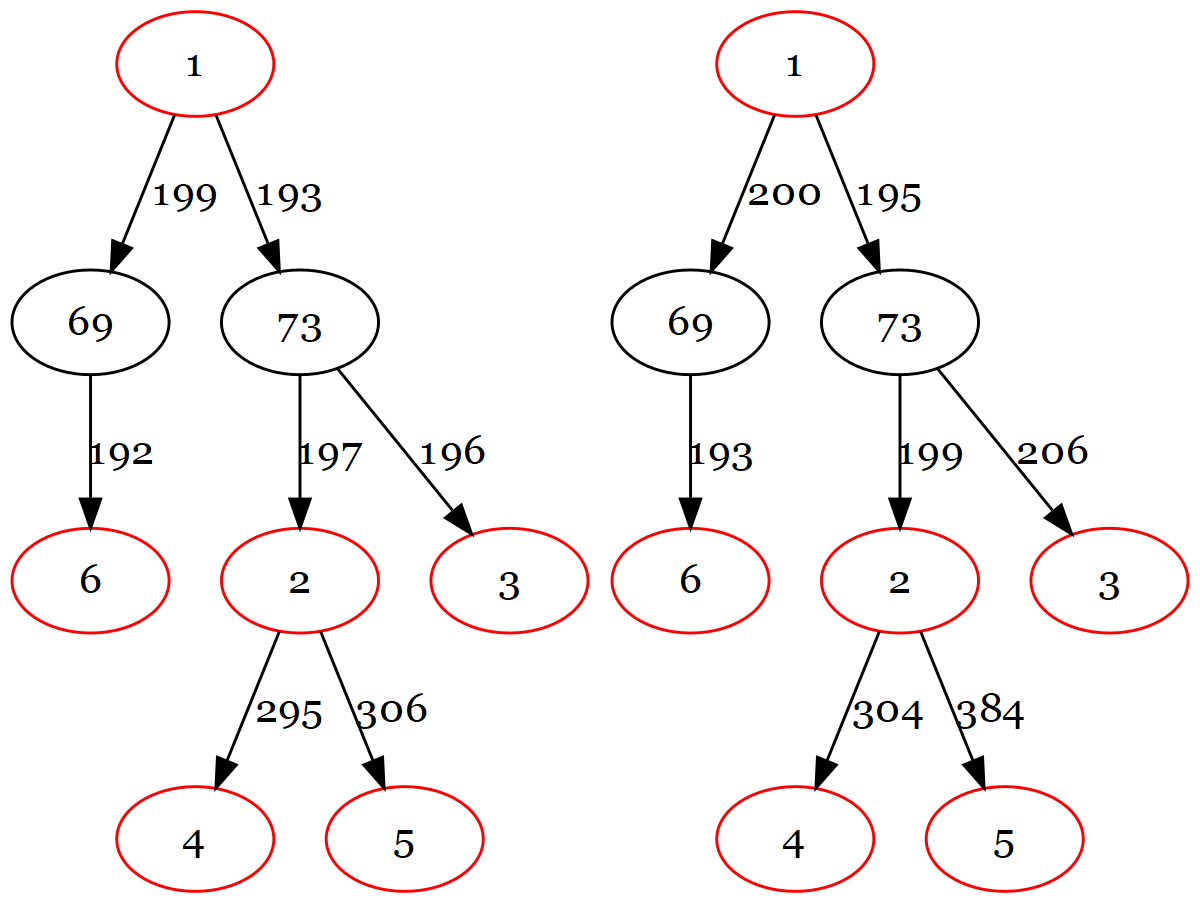
\includegraphics[scale=0.25]{figures/crit.png}
\caption{Output tree of testcase 41(left) and critical payments(right)}\label{fig:crit41}
\end{figure}
 
We can clearly see that most of these critical payments are just slightly higher, than the original cost. This is because there are a lot of other viable options in the graph we used, which was testcase 41. If there is an edge in the graph, that is irreplaceable e.g. if there is a terminal that has a degree of one within the graph, then its critical payment would be $\infty$, since it would always be included in the solution tree, no matter how high its cost. Now knowing the critical payments we can easily adjust our implementation of the Berman, Ramaiyer algorithm to always pay out the critical payment to the winning seller, which makes out algorithm implement critical payments. We could do this just as well with the MST-approximation or with the $IRGH$-algorithm. If we look at the results presented in Appendix \ref{chapter:appendix} we can see that for the MST-approximation and Berman, Ramaiyer the total critical payments are always greater than the total original cost. This is the expected behaviour and is due to the monotonicity breaking cases in this algorithms appearing very rarely, as opposed to $IRGH$, where in every tested case the total critical payments were less than the original cost. This is a strong indication that the critical payments of $IRGH$ are very unreliable.


\section{Incentive Compatibility}

Using the Lemma by Blumrosen and Nisan \cite{BlNi07} we can conclude that MST-approximation algorithm, as well as the algorithm by Berman and Ramaiyer, are incentive compatible or strategy proof after modifying them so that critical payments are payed out to the winning seller, regardless of the price offered to us. Hougardy and Proemel's $IRGH$ algorithm does not implement monotonicity so we can use the aforementioned Lemma to disprove incentive compatibility for $IRGH$. Since we have proven strategy proofness for Berman, Ramaiyer's algorithm, we can assume that the valuations that the sellers give us reflect their true valuations of the edges which they are selling to us. 